% Packages utilisés :
%
% \usepackage[french]{babel}
% \usepackage[utf8x]{inputenc}
% \usepackage{amsmath}
% \usepackage{amssymb}
% \usepackage{tikz}
% \usepackage{tkz-graph}
%
% Il y a aussi besoin d'un environnement solution

\section{Séance 3}

\begin{solution}
	Étant donné que cet algorithme doit, au plus, parcourir toutes les arêtes pour trouver le chemin, on a une complexité en $O(\vert E \vert)$, avec $\vert E \vert$ le nombre d'arêtes dans le graphe.\\

	Le pire des cas (celui où le nombre d'arêtes est le plus élevé) est le cas du graphe complet. En effet, par le théorème des poignées de mains, on a que $\vert E \vert = \frac{n(n-1)}{2}$. La complexité est donc $O(n^2)$, avec $n$ le nombre de nœuds dans le graphe.
\end{solution}

\paragraph{2. } Lorsque certaines longueurs dans un digraphe sont négatives il peut être nécessaire de devoir faire la distinction entre la plus courte chaîne et le plus court chemin. Donnez l'exemple d'un graphe pour lequel cette distinction est nécessaire. Cette distinction est-elle nécessaire si tous les circuits sont de longueur positive?


\begin{solution}
Une chaine \footnote{même chose qu'un parcours} est une suite $v_0e_1v_1e_2...e_nv_n $ où $v_1,v_2,...$ sont des sommets et $e_1,e_2,...$ sont des arêtes. 
Un chemin est une chaine dont les sommets sont tous distincts.\\

Si on veut trouver le chemin de poids minimum de A à E, on a ABDE de poids $8$. Par contre le poids optimum de la chaîne n'a pas de borne inférieure car la chaîne peut passer une infinité de fois sur les arêtes de poids négatif.\\
\begin{figure}[h!]
\centering
\begin{tikzpicture}[scale=0.75,transform shape]
  \Vertex[x=-6,y=0]{A}
  \Vertex[x=-3,y=0]{B}
  \Vertex[x=0,y=-4]{C}
  \Vertex[x=0,y=4]{D}
  \Vertex[x=6,y=0]{E}
  \tikzset{LabelStyle/.style =   {draw}}
  \tikzstyle{EdgeStyle}=[]
  \Edge[label=$20$](A)(B)
  \Edge[label=$-5$](B)(C)
  \Edge[label=$-15$](D)(B)
 \Edge[label=$2$](C)(D)
  \Edge[label=$3$](D)(E)
\end{tikzpicture}
\end{figure}

Preuve : par l'absurde\\
Supposons que la plus courte chaîne et le plus court chemin sont différents. Il y a deux possibilités :
- Soit le plus court chemin est plus court ou égal à la plus courte chaîne. Dans ce cas, il existe une plus courte chaîne que celle trouvée précédemment, c'est à dire le plus court chemin.\\
- Soit la plus courte chaine est plus courte que le plus court chemin. Nous savons que pour qu'une chaîne soit la plus courte entre u et v, il faut qu'elle soit aussi la plus courte entre deux nœuds intermédiaires du graphe, supposons que le cycle comprenne deux fois le nœud w, pour que la chaîne soit optimale, il faut que le chemin entre w et w soit optimal, or le cycle a une longueur strictement positive, on peut donc trouver un chemin plus court entre w et w de taille 0(ne pas faire le cycle). La chaîne trouvée précédemment n' est donc pas optimale, on obtient donc une contradiction, on utilise le même argument pour tout les cycles du graphes.
\end{solution}



\paragraph{5. } Le graphe dirigé ci-dessous est acyclique. Utilisez l'algorithme de Dijkstra pour trouver le plus court chemin du noeud $1$ à chaque autre noeud du graphe.
\begin{solution}
\begin{center}
  \begin{tikzpicture}[->,>=stealth',shorten >=1pt,auto]
    \Vertex[x=0 ,y=0]{1}
    \Vertex[x=0 ,y=-2]{4}
    \Vertex[x=2,y=1]{2}
    \Vertex[x=2 ,y=-1]{3}
    \Vertex[x=2 ,y=-3]{7}
    \Vertex[x=4 ,y=0]{5}
    \Vertex[x=4 ,y=-2]{6}

    \path[every node/.style={font=\sffamily\small}]
    (1) edge node [left] {12} (2)
    edge node [left] {4} (4)

    (2) edge node [right] {5} (5)

    (3) edge node [right] {4} (2)
    edge node [left] {7} (5)
    edge node [right] {3} (7)

    (4) edge node [left] {3} (3)
    edge node [right] {4} (7)

    (5) edge node [right] {3} (6)

    (7) edge node [left] {9} (6);

  \end{tikzpicture}
\end{center}

	Premièrement, un exemple où il n'existe pas de parcours du nœud $0$ au nœud $p$ avec $p=3$ et $a_1 = 2$. En effet, il n'est pas possible d'échanger $3$ euros avec des pièces de $2$ euros.\\

\paragraph{6. } Vous avez deux seaux d'une contenance de 7 et 5 litres. Vous avez besoin de 4 litres. Les opérations permises sont les suivantes : remplir un seau, vider un seau, verser le contenu d'un seau dans l'autre jusqu'à ce que le seau soit rempli ou l'autre vide. Vous souhaitez effectuer un nombre minimum d'opérations et obtenir un seau contenant 4 litres. Formulez ce problème comme un problème de plus court chemin, et trouvez-en la solution.

\begin{solution}
Le problème peut être modélisé comme le plus court chemin entre le nœud (0,0) et (0,4) dans le graphe donné. Il suffit de suivre la chaîne, on obtient sept opérations nécessaires. Nous n'avons tracé que les arêtes permettant d'allant dans les deux sens, par exemple, nous n'avons pas tracer  l'arête entre (5;4) et (5;0) car on peut aller de (5;4) à (5;0) mais pas de (5;0) à (5;4). On peut constater que le chemin le plus court est de 7 opérations. Il est tracé en rouge.
\begin{figure}[h!]
\centering
\begin{tikzpicture}[scale=0.75,transform shape]
  \Vertex[x=-10,y=0]{0;0}
  \Vertex[x=-8,y=2]{0;7}
  \Vertex[x=-8,y=-2]{5;0}
  \Vertex[x=-6,y=2]{5;2}
  \Vertex[x=-6,y=-2]{0;5}
  \Vertex[x=-4,y=2]{0;2}
  \Vertex[x=-4,y=-2]{5;5}
  \Vertex[x=-2,y=2]{2;0}
  \Vertex[x=-2,y=-2]{3;7}
  \Vertex[x=0,y=2]{2;7}
  \Vertex[x=0,y=-2]{3;0}
  \Vertex[x=2,y=2]{5;4}
  \Vertex[x=2,y=-2]{0;3}
  \Vertex[x=4,y=2]{0;4}
  \Vertex[x=4,y=-2]{5;3}
  \Vertex[x=6,y=2]{4;0}
  \Vertex[x=6,y=-2]{1;7}
  \Vertex[x=8,y=2]{4;7}
  \Vertex[x=8,y=-2]{1;0}
  \Vertex[x=10,y=2]{5;6}
  \Vertex[x=10,y=-2]{0;1}
   \Vertex[x=12,y=2]{0;6}
  \Vertex[x=12,y=-2]{5;1}
  \tikzset{LabelStyle/.style =   {draw}}
  %\tikzstyle{LabelStyle}=[fill=white,sloped]
  \tikzstyle{EdgeStyle}=[double = red]
  \Edge(4;0)(0;4)
  \Edge(0;4)(5;4)
  \Edge(5;4)(2;7)
 \Edge(2;7)(2;0)
  \Edge(2;0)(0;2)
  \Edge(0;2)(5;2)
 \Edge(5;2)(0;7)
  \Edge(0;7)(0;0)
  \tikzstyle{EdgeStyle}=[]
    \Edge(0;0)(5;0)
  \Edge(5;0)(0;5)
  \Edge(0;5)(5;5)
 \Edge(5;5)(3;7)
  \Edge(3;7)(3;0)
  \Edge(3;0)(0;3)
  \Edge(0;3)(5;3)
  \Edge(5;3)(1;7)
 \Edge(1;7)(1;0)
  \Edge(1;0)(0;1)
  \Edge(0;1)(5;1)
  \Edge(5;1)(0;6)
  \Edge(0;6)(5;6)
 \Edge(5;6)(4;7)
  \Edge(4;7)(4;0)
\end{tikzpicture}
\end{figure}
\end{solution}

\paragraph{7. }
	Vous possédez un billet de $p$ euros et vous souhaitez le changer en pièces de $a_1, a_2, ..., a_k$ euros (tous les montants étant entiers). Est-ce possible? Si oui, avec quel nombre de pièces? Formulez ce problème comme un problème de plus court chemin dans un graphe.


\begin{solution}
	Créons un digraphe de la manière suivante : $p+1$ nœuds numéroté de $0$ à $p$ et des arêtes telles qu'une arête associée à une pièce de valeur $a_k$ relie un nœud $i$ à un nœud $i+a_k$\footnote{à condition de ces deux nœuds à relier soient bien compris entre $0$ et $p$}. Il suffit ensuite d'appliquer l'algorithme de Dijkstra au graphe créé pour chercher le plus petit chemin entre les nœuds $0$ et $p$. Si l'algorithme ne trouve pas de chemin, il est alors impossible d'échanger le montant $p$ avec les pièces disponibles. Vous pouvez regarder quelques exemples ci-dessous.\\
\begin{center}
	\begin{tikzpicture}[scale=0.75,transform shape]
		\Vertex[x=-10,y=0]{0}
 		\Vertex[x=-8,y=0]{1}
		\Vertex[x=-6,y=0]{2}
		\Vertex[x=-4,y=0]{3}
		\tikzset{LabelStyle/.style =   {draw}}
	 	\tikzstyle{EdgeStyle}=[bend left]
	 	\Edge(0)(2)
	 	\tikzstyle{EdgeStyle}=[bend right]
		\Edge(1)(3)
 	\end{tikzpicture}
\end{center}

	Deuxièmement, un exemple ou il existe un parcours de $0$ à $p$ avec $p=5$, $a_1=2$ et $a_2=1$. Le chemin le plus court est tracé en rouge et correspond à $2$ pièces de $2$ et une pièce de $1$. Il existe deux autres chemins de même longueur (donc équivalents).\\

\begin{center}
	\begin{tikzpicture}[scale=0.75,transform shape]
		\Vertex[x=-10,y=0]{0}
		\Vertex[x=-8,y=0]{1}
		\Vertex[x=-6,y=0]{2}
		\Vertex[x=-4,y=0]{3}
		\Vertex[x=-2,y=0]{4}
		\Vertex[x=0,y=0]{5}
		\tikzset{LabelStyle/.style =   {draw}}
		\tikzstyle{EdgeStyle}=[bend left,double=red]
		\Edge(0)(1)
		\tikzstyle{EdgeStyle}=[bend left]
		\Edge(1)(2)
		\Edge(2)(3)
		\Edge(3)(4)
		\Edge(4)(5)
		\tikzstyle{EdgeStyle}=[bend right, double = red]
		\Edge(1)(3)
		\Edge(3)(5)
		\tikzstyle{EdgeStyle}=[bend right]
		\Edge(0)(2)
	  	\Edge(2)(4)
 	\end{tikzpicture}
\end{center}

\end{solution}
La matrice associée à l'algorithme de Dijkstra est donnée par : 
\[\mathcal{D}= 
\left(\begin{array}{ccccccc}
1 & 2   & 3       & 4  & 5          & 6 & 7 \\
\boxed{0} & 12 & \infty & 4 & \infty    &\infty & \infty  \\
\boxed{0} & 12 & 7       & \boxed{4} & \infty    & \infty  & 8  \\
\boxed{0} & 11 & \boxed{7}       &\boxed{4} & 14         & \infty  & 8\\
\boxed{0} & 11 & \boxed{7}       & \boxed{4}& 14         & 17 & \boxed{8}\\
\boxed{0} & \boxed{11} & \boxed{7}       & \boxed{4} & 14         & 17 &  \boxed{8}\\
\boxed{0} & \boxed{11} & \boxed{7}      & \boxed{4} & \boxed{14}         & 17 &  \boxed{8}\\
\boxed{0} & \boxed{11}& \boxed{7}       & \boxed{4} & \boxed{14}         & \boxed{17} &  \boxed{8}\\
\end{array}\right)\]

\end{solution}

